\section{Análisis del Sistema}
	Se requiere un Sistema de Salud Ocupacional donde se puedan registrar
	empresas, pacientes (asociados o no a una empresa) que, deben ser sometidos a
	pruebas médicas de acuerdo a un perfil de exámenes previamente registrados.
	Terminada las pruebas, el sistema debe imprimir dichas pruebas junto con los
	datos calculados automáticamente.\footnote{El párrafo es un resumen del
	documento de requerimientos real.} \\\

	A continuación se muestran algunos diagramas:
	
	\begin{figure}[ht!]
	    \centering
		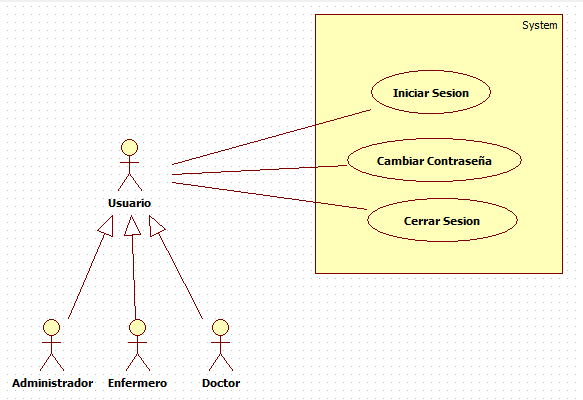
\includegraphics{../imgs/casos-uso/1.png}
		\caption{CU-1 Seguridad}
	\end{figure}
	
\newpage
	
	\begin{figure}[ht!]
	    \centering
		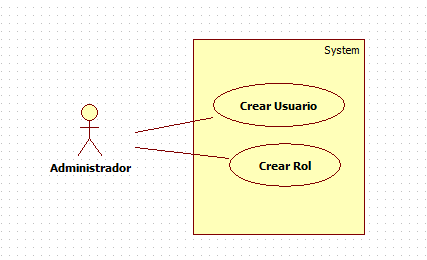
\includegraphics{../imgs/casos-uso/2.png}
		\caption{CU-2 Creación de Usuarios}
	\end{figure}
	
	\begin{figure}[ht!]
	    \centering
		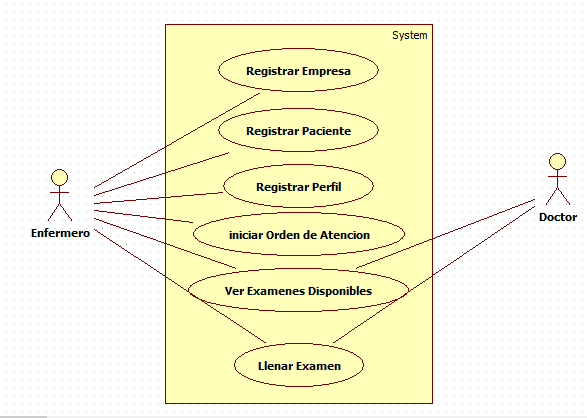
\includegraphics{../imgs/casos-uso/3.png}
		\caption{CU-3 Casos de Uso primordiales}
	\end{figure}